%%%%%%%%%%%%%%%%%%%%%%%%%%%%%%%%%%%%%%%%%%%%%%%%%%%%%%%%%
%  PATT2 FORM VERSION 02/2003 - TEMPLATE                %
%%%%%%%%%%%%%%%%%%%%%%%%%%%%%%%%%%%%%%%%%%%%%%%%%%%%%%%%%
%  ENTER THE INFORMATION BETWEEN THE CURLY BRACKETS     %
%%%%%%%%%%%%%%%%%%%%%%%%%%%%%%%%%%%%%%%%%%%%%%%%%%%%%%%%%
%  DO NOT EDIT THE PATT2.STY FILE IN ANY WAY            %
%%%%%%%%%%%%%%%%%%%%%%%%%%%%%%%%%%%%%%%%%%%%%%%%%%%%%%%%%

%%%%%%%%%%%%%%%%%%%%%%%%%%%%%%%%%%%%%%%%%%%%%%%%%%%%%%%%%
% the default font size must not be altered from 11pt.  %
% proposals written in a smaller font will be rejected  %
%%%%%%%%%%%%%%%%%%%%%%%%%%%%%%%%%%%%%%%%%%%%%%%%%%%%%%%%%
                                                       
\documentclass[11pt]{article}
\usepackage{patt2}

% Allow epsfig, psfig or graphicx packages

\usepackage{epsfig}
\usepackage{psfig}
\usepackage{graphicx}
\usepackage{natbib}

% Uncomment below if using pdflatex
\usepackage{epstopdf}
\pdfpageheight=11.69in
\pdfpagewidth=8.26in

\typeout{This is the PATT2 (Optical/IR) blank LaTeX form}

% add any personal macros here

% end macros

\begin{document}

\telescope{WHT}    % AAT, UKST, WHT, INT or UKIRT
\semester {2020B}    % eg 2003B

\category {4}    % Scientific Category (enter a number):
                % 1 Solar system and extrasolar planets
                % 2 ISM, CSM, PNe, including star formation
                % 3 Stars and stellar populations (galactic and circum-galactic)
                % 4 Low-z universe
                % 5 High-z universe
 
\relatedapps {}{}{}{}{}{}{}{}{} % Coordinated PATT applications {x}
% in order  AAT,UKST,WHT,INT,UKIRT,JCMT,Gemini,LT,MERLIN

%%%%%%%%%%%%%%%%%%%%%%%%
% PAGE 1 OF PATT2 FORM %
%%%%%%%%%%%%%%%%%%%%%%%%

% PI information

\pisurname     {Lintott}                % Surname
\pititle       {Prof}                % Mr/Mrs/Ms/Miss/Dr/Prof
\pifirstname   {Chris}                % First name
\pistatus      {Professor of Astrophysics/Citizen Science Lead}                % Post held
\piaddressone  {University of Oxford}                % Name of Institute
\piaddresstwo  {Department of Astrophysics, Denys Wilkinson Building}                % Postal Address
\piaddressthree{Keble Road, Oxford, OX1 3RH, UK}                % Postal Address
\piphone       {00441865273638}                % Phone number
\pifax         {}                % Fax number
\piemail       {chris.lintott@physics.ox.ac.uk}                % email address
\piobserver    {Yes}                % Is the PI going to observe? {Yes/No}

% collaborator 1

\collabonename    {Dr Rebecca Smethurst}             % Name of first collaborator
\collaboneinst    {University of Oxford}             % Name of Institute
\collaboneobserver{Yes}             % Will collaborator observe? {Yes/No}

% collaborator 2

\collabtwoname    {Mr Tobias Geron}
\collabtwoinst    {University of Oxford}
\collabtwoobserver{Yes}

% collaborator 3

\collabthreename    {Dr Brooke Simmons}
\collabthreeinst    {Lancaster University}
\collabthreeobserver{No}

% collaborator 4

\collabfourname    {}
\collabfourinst    {}
\collabfourobserver{}

% note additional collaborators can be added by inserting multiple
%names into these entries.



% proposal information 

\title      {Are weak bars the progenitors of strong bars?}                % Brief title  (12 words only)

\abstract   {We will do great science. Huge. 

% summary of proposed observations
% add your abstract here.  the font size must not be smaller 
% than the default in the style-file


}                


% Instrument requirements

\focalstation       {f/11}        % eg prime,f/3.3,f/8,f/15,f/36,cs/36
\instrument         {ISIS}        % eg RGO spec, UCLES, UHRF, Taurus, TTF, IRIS
                              % prime focus imager, LDSS etc
\detector           {EEV12, RED+}        % which chip do you want to use?
\gratingsandfilters {R300B, R316R}        % eg UBVRI,H$\alpha$,1200R,etc

\timerequested  {3}{}{}{Nights}      % No. of {Dark},{Grey},{Bright}, 
                              % {Weeks/Nights/Hours}
\minuseful      {3}{}{}        % Minimum number of useful {D},{G},{B} 
\lttotaltime    {}{}{}{}      % For long term proposals indicate the
                              % TOTAL requested {D},{G},{B},{W/N/H}


%%%%%%%%%%%%%%%%%%%%%%%%
% PAGE 2 OF PATT2 FORM %
%%%%%%%%%%%%%%%%%%%%%%%%

\prefdates            {Autumn}      % Preferred dates, eg Jan,Feb
\impossdates          {}      % Impossible dates, eg Mar,Apr
\datesjustification   {Wrong RAs}      % Why impossible? eg wrong RAs, etc
\simultaneous         {}      % Simultaneous with other tels/satellites?
\othertimeconstraints {}      % eg Moon phase/position,specific dates
\serviceobservingyes  {}      % Observations to be done as Service? {x}
\serviceobservingno   {}      % or not {x}
\serviceobservingmaybe{}      % or maybe {x}
\supporteverynight    {}      % Support astronomer every night? {x}
\supportnone          {}      % No support astronomer? {x}
\supportfirstnight    {x}      % Support astronomer first night only? {x}
                              % (This is the only option for ING)

% target info                 % Target RA,Dec,Mags,Colours,Exp Time

\targetinfo{

%enter target information here.  this should include name, ra, dec
%and some indication of magnitude, line flux etc.  it is OK to use
%a small font here.

}

% LIST ALL SIMILAR/SUPPORTING APPLICATIONS TO ANY PATT OR OTHER TIME
% ASSIGNMENT COMMITTEE  
% You must include a brief description of any
% other applications whose targets or science goals are similar to 
% those requested here

\otherapplications{
\begin{tabular}[t]{p{1.6in}p{5.0in}}
%Telescope/Committee & Short title of programme  \\
\end{tabular}
}


%%%%%%%%%%%%%%%%%%%%%%%%%%%%%%%%%%%%%%%%%%%%%%%%%%%
% PAGE 3 OF PATT2 FORM - SCIENTIFIC JUSTIFICATION %
%%%%%%%%%%%%%%%%%%%%%%%%%%%%%%%%%%%%%%%%%%%%%%%%%%%

\sciencecase{

Understanding the role that internal processes play in galaxy evolution is a key goal of modern astrophysics. An increasing body of evidence shows that galaxy growth is mainly dependent on such processes rather than galaxy mergers; \citet{kaviraj12}, for example, have shown that only 27\% of star formation is triggered by major or minor mergers. The focus has therefore shifted to trying to determine the dominant mechanisms responsible for galaxy growth and the quenching (or cessation) of star formation. One such process is the funneling of gas from the outskirts of a galaxy by a galactic-scale bar. Bars are thought to remove gas needed for star formation in the outer regions and deposit it in the centre where it either triggers a starburst or is too dynamically hot to be used for future star formation. In either the case, the eventual result is thought to be that the galaxy has a lower star formation rate than before the formation of the bar, moving the galaxy from the blue cloud to the red sequence. 

One question that remains unanswered however is whether this only occurs in the strongest of barred galaxies, where the bar is the dominant feature. A large range of bar strengths is seen across the galaxy population with a broad distribution of bar lengths, widths and relative sizes (see Figure~\ref{fig:histograms}). Most previous studies have focussed their efforts on the strong bar population which are easier to select from galaxy surveys since they are brighter and constitute the main feature of the galaxy. In contrast, there are a few studies which then specifically target weaker bars to determine their effects on the galaxy. However, it is not known if weak and strong bars are a dichotomy in the barred galaxy population or a continuous distribution of the same feature with similar effects. 

In this project we propose to observe a mass-matched sample of strong and weak bars along with a control sample of no bars in order to characterise the effects of bars and the impact of strong and weak bars. We will use the ISIS spectrograph on the WHT to obtain spectra along and perpendicular to the bar for each target (unbarred galaxies will have the slit aligned along the major and minor axes). The flexibility provided by the choice in gratings makes ISIS the ideal instrument to achieve our science goals. In particular, resolving the emission lines in each target across a large range of wavelengths will allow us to determine the gas kinematics along and perpendicular to the bar.  We aim to test whether there is a significant inflow of gas along the bar, compared to outside the bar (and the control sample of unbarred galaxies) and therefore whether bars are indeed a significant driver of galaxy evolution. Complementary to this we will test whether there is a significant difference in the gas kinematics of strong and weak bars in order to determine if weak bars are a separate phenomenon to strong bars or part of a continuous distribution. Do weak bars drive gas to the centre of a galaxy at the same or different rates to strong bars?

The simultaneous observation of both the blue and red side of the spectrum with IDIS will also allow us to determine the star formation rates within and outside the bar using $H\alpha$ on the red side, and $Dn4000\AA$ & \textsc{[OIII]} on the blue side. These resolved star formation rates will be crucial to determining if the bar is indeed responsible for any change in the star formation rate in these galaxies. Once again we will also test the differences between the resolved star formation rates of strong and weak bars to determine whether both types of structures are able to quench the star formation in a galaxy. 

We aim to publish two papers as a result of these observations: (1) determining the gas kinematics for each of our targets to determine which structures (if any) are inflowing gas to the centres and (2) constraining the star formation rates inside and outside of the bar to determine whether either strong or weak bars are directly responsible for quenching galaxies.

% add your science case here.  

% proposals written in a font smaller than 11pt will be rejected

}

%%%%%%%%%%%%%%%%%%%%%%%%%%%%%%%%%%%%%%%%%%%%%%%%%%%%%%%%
% PAGE 3a OF PATT2 FORM - SCIENTIFIC JUSTIFICATION     %
% FOR PROPOSALS TO AAT, WHT or UKIRT FOR 8 OR MORE     % 
% NIGHTS, AND FOR  ALL (I.E. INCLUDING INT AND UKST)   %
% LONG-TERM AND COORDINATED PROPOSALS (INCLUDING THOSE %
% COORDINATED WITH NON-PATT TELESCOPES)                %
%%%%%%%%%%%%%%%%%%%%%%%%%%%%%%%%%%%%%%%%%%%%%%%%%%%%%%%%

\extendedsciencecase{

% continue your science case here ONLY if applying for 8 or 
% more nights to the AAT, WHT OR UKIRT, or if your proposal 
% is a long-term (multi-semester) proposal to the AAT, UKST, 
% WHT, INT or UKIRT, or if your proposal (to AAT, UKST, WHT, 
% INT or UKIRT) is coordinated with other telescopes (including 
% non-PATT telescopes).  

% Remember to comment IN the \makepatttwopagethreea command later 
% in this file if you have written an extended science case  

% proposals written in a font smaller than 11pt will be rejected

}


%%%%%%%%%%%%%%%%%%%%%%%%%%%%%%%%%%%%%%%%%%%%%%%%%%%%%%%%%%%%%%%%%%%%%%%%%%%%
% PAGE 4 OF PATT2 FORM - TECHNICAL INFORMATION (I) - FEASIBILITY, S/N, ETC %
%%%%%%%%%%%%%%%%%%%%%%%%%%%%%%%%%%%%%%%%%%%%%%%%%%%%%%%%%%%%%%%%%%%%%%%%%%%%

\technicalpage{
PARAGRAPH FROM TOBIAS ABOUT SAMPLE SELECTION. 

The ISIS spectrograph on the WHT is ideal for observing this sample as it allows the simultaneous observation of the red and blue sides of the spectrum in combination with the felxibility of the gratings available. This allows us to optimise the wavelength range targetted against the spectral resolution in order to maximise the science output. We therefore propose to target the $H\alpha$ emission line in each of our sources with the R316B grating on the RED+ detector, with simultanous observations of the $D_n4000\AA$ break-$H\beta$-\textsc{[OIII]} region using the R300B on the EEV12 detector. Probing these regions of the spectrum specifically will allow us to observe a maximum number of emission lines to derive precise gas kinematics whilst also allowing for an accurate determination of the resolved star formation rate in and outside the bar. 

In order to derive an accurate measure of the gas inflow rates in our targets, we need to be able to determine the gas kinematics. We will utilise the tried and tested \textsc{ppxf} spectral fitting code \citep{cappellari04} to derive the velocity of the gas along the bar for each of our targets. To do this we require a high signal-to-noise ratio (SNR) to ensure that each of the emission lines in the sample are well resolved. To achieve a $SNR=10$ for each of our targets we calculated an exposure time given the quantum efficiency of the detectors at the redshifted wavelegnth of $H\alpha$ and assuming negligible sky background on dark sky nights with respect to the read noise of the EEV12 and RED+ detectors. Given these requirements the total on source time is ??? minutes, assuming a seeing of 1" and optimal airmass conditions. The minimum (maxmimum) exposure time for a single source is ?? (??) minutes. 

Using this information combined with the overhead estimates from the ISIS Total Observing Time Estimator and assuming an average weather downtime of ??\% in ??, we calculate that we can observe all 30 targets in ?? nights of dark skies in ?? of the 2020 semester. 

% add any technical details you wish to transmit to the panel and
% technical assessor here. you may also include references here
% as well as on the next page

% proposals written in a font smaller than 11pt will be rejected


}

%%%%%%%%%%%%%%%%%%%%%%%%%%%%%%%%%%%%%%%%%%%%%%%%%%%%%%%%%%%%%%%%%%%%%%%%%%%%%%
% PAGE 4a OF PATT2 FORM - TECHNICAL INFORMATION (II) - REFERENCES, FIGS, ETC %
%%%%%%%%%%%%%%%%%%%%%%%%%%%%%%%%%%%%%%%%%%%%%%%%%%%%%%%%%%%%%%%%%%%%%%%%%%%%%%

\figsandrefspage{

% \begin{bibliography}
% \bibliographystyle{astron}% add any figures, references etc here.  remember to embed your figures.
% \end{bibliography}
% \epsfxsize
% \hsize
% \epsffile{mosaic.ps}
\centering{
\psfig{file=mosaic.pdf,width=17cm}\label{fig:mosaic}
Figure 1: Mosaic of SDSS postage stamps of sample. Strong bars (top), weak bars (middle) and no bars (bottom) with surface brightness shown.
}

\centering{
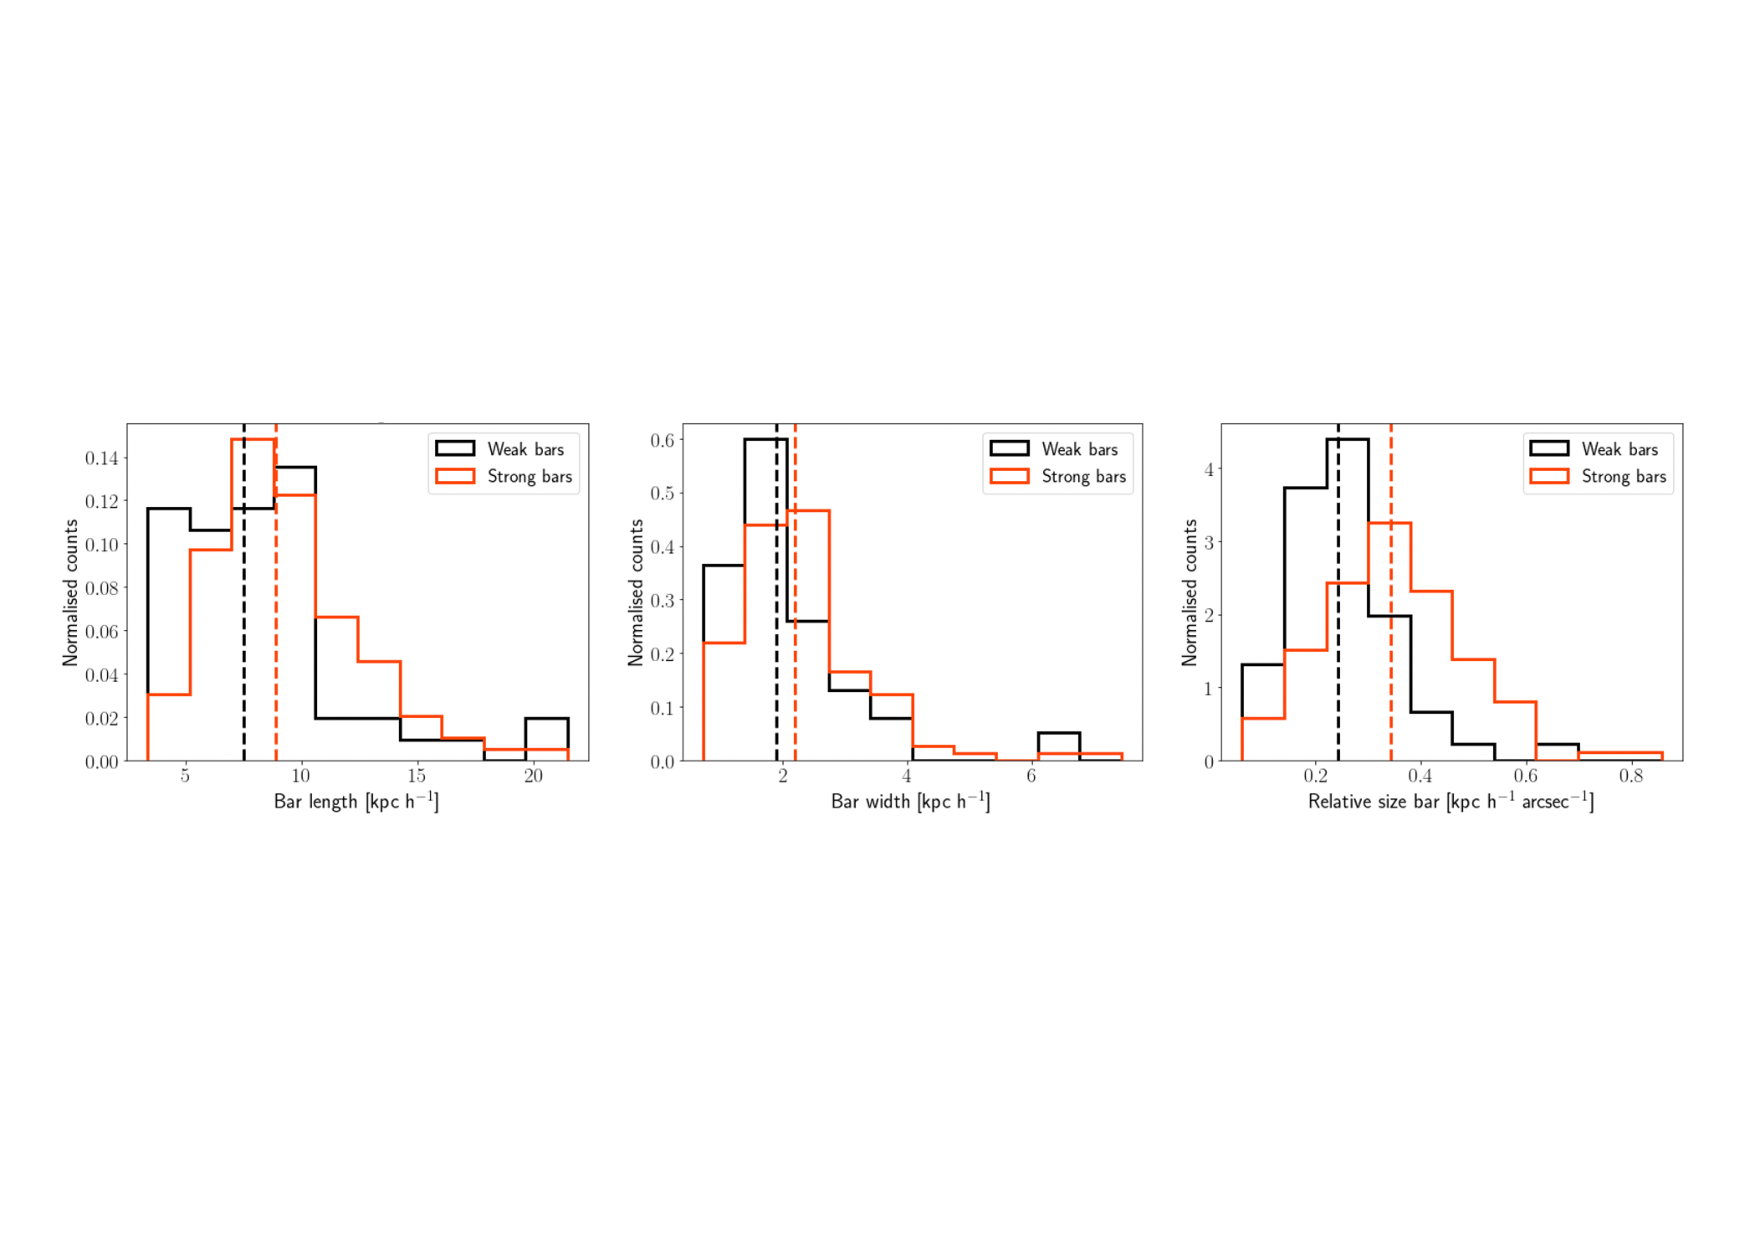
\psfig{file=histograms.pdf,width=17cm}\label{fig:histograms}
Figure 2: Histograms showing bar properties.}

\centering{
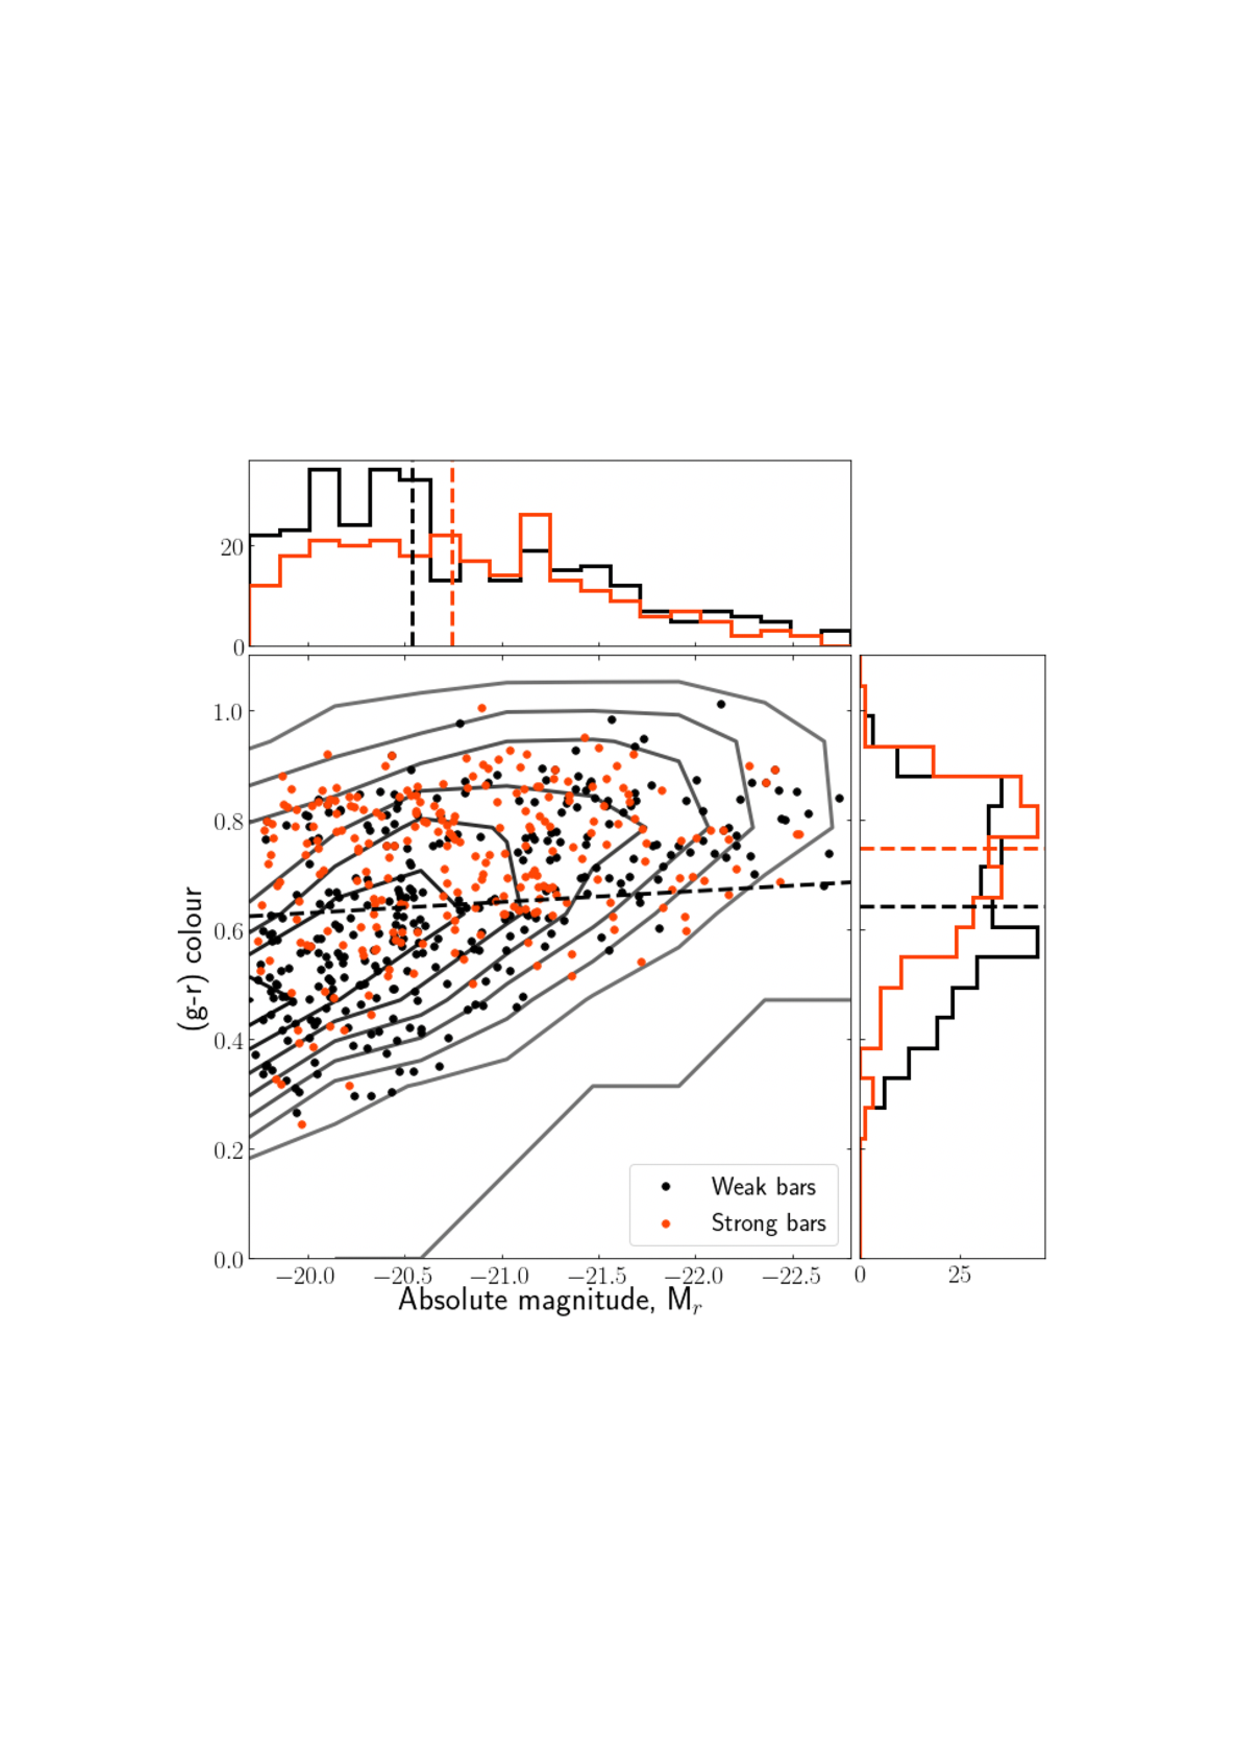
\psfig{file=colour_mag_diagram.pdf,width=7.5cm}\label{fig:colmag}
Figure 3: Colour magnitude diagram suggesting strong and weak bars are separate populations, with strong bars causing quenching.}


% proposals written in a font smaller than 11pt will be rejected

}

%%%%%%%%%%%%%%%%%%%%%%%%
% PAGE 5 OF PATT2 FORM %
%%%%%%%%%%%%%%%%%%%%%%%%

\backupprogram{}             % Summary of backup programme

\previous{                   % Previous applications (last 4 Sems)
\begin{tabular}[t]{p{1.5in}p{0.7in}p{0.8in}p{3.2in}}
%Patt No. & Award & clear nights & comments \\
\end{tabular}
}

\publications     {}         % List pubs with data from patt time (last 4 Sems)

\experience       {}         % Experience of observers on other telescopes
\graduatestudent  {}{}       % Research student {Name of student}{Project}
\grant            {}{}{}     % {Name of PI}{Grant title}{Grant No.}
\nonstandardtravel{}         % Justify T&S for more than one UK observer
\otherexpenditure {}         % eg for freight etc.


%%%%%%%%%%%%%%%%%%%%%%%%%%%%%%%%%%%%%%%%%%%%%%%%%%%%%%%%%%%%%%%%%%%%%%%%%%%%%
% PAGE 6 OF PATT2 FORM - THIS SECTION IS REMOVED BY THE AAT DURING PROCESSING
% IF INCLUDED.  ING APPLICANTS SHOULD NOT ENTER ANYTHING HERE.
%%%%%%%%%%%%%%%%%%%%%%%%%%%%%%%%%%%%%%%%%%%%%%%%%%%%%%%%%%%%%%%%%%%%%%%%%%%%%

\shorttitle {}               % Ignore if you are an ING applicant.



\makepatttwopageone
\makepatttwopagetwo
\makepatttwopagethree

%%%%%%%%%%%%%%%%%%%%%%%%%%%%%%%%%%%%%%%%%%%%%%%%%%%%%%%%%%%%%%%%%%%%%
% COMMENT THE FOLLOWING LINE IN *ONLY* IF                           % 
%                                                                   %
% YOU ARE APPLYING FOR 8 OR MORE NIGHTS ON THE AAT, WHT OR UKIRT, OR% 
% YOUR PROPOSAL IS LONG-TERM FOR THE AAT, WHT, UKIRT OR INT, OR     % 
% YOUR PROPOSAL IS COORDINATED WITH OTHER TELESCOPES                % 
%                                                                   % 
% *AND* YOU HAVE USED THE CONTINUATION PAGE FOR YOUR SCIENTIFIC CASE% 
%%%%%%%%%%%%%%%%%%%%%%%%%%%%%%%%%%%%%%%%%%%%%%%%%%%%%%%%%%%%%%%%%%%%%
 
\makepatttwopagethreea

\makepatttwopagefour
\makepatttwopagefoura
\makepatttwopagefive

% FOR ING APPLICATIONS LEAVE THE FOLLOWING LINE COMMENTED OUT

%\makepatttwopagesix         

% FOR AAT APPLICATIONS YOU MAY LEAVE IT IN IF YOU WISH.  IT WILL NOT
% BE TRANSMITTED TO THE TAG HOWEVER.

\end{document}
